% Multiple linear regression
% Standardized coefficients
% Regression dummies
% Regression diagnostics

\documentclass[t]{beamer}
\usetheme{\usetheme{hkllite}}

\title{linear regression}
	\author{François Briatte \& Ivaylo Petev}
	\date{Week~\#10}

\graphicspath{{images/}}

\begin{document}
    

    % disable footline on title page
    \frame[plain]{
        \titlepage\\[7em]
        \tableofcontents[hideallsubsections]
        }

    
		%
		%

    \section{Multiple linear regression}

	\begin{frame}[c]%{Multiple linear regression}
			
		\begin{center}
			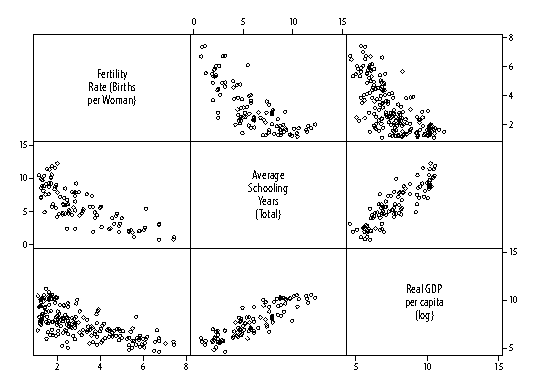
\includegraphics[width=\textwidth]{mreg-gr-mat.pdf}
		\end{center}
				
	\end{frame}
	
	\begin{frame}[c]{Multiple linear regression} % or, as my girlfriend calls it, ultimate regression
			
		\begin{center}
			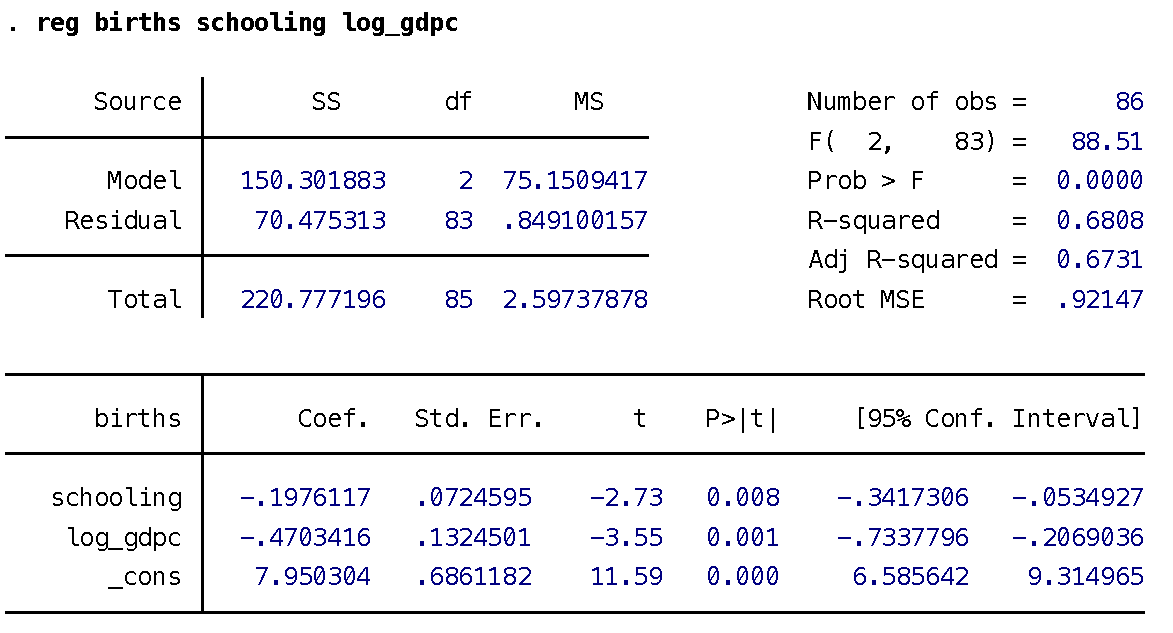
\includegraphics[width=\textwidth]{mreg-output.pdf}
		\end{center}
				
	\end{frame}	
	
	\begin{frame}[c]{Multiple linear regression}
		
		$$Y = \alpha+\beta_1 X_1+\beta_2 X_2+,\ldots,+\beta_k X_k+\epsilon$$
		
		\vfill
		 
		\begin{block}{Partial derivatives}

			Each coefficient is calculated by \red{holding all others constant}.

		\end{block}

		\begin{block}{Least squares}

			The model is still optimized by minimizing the squared error terms.

		\end{block}

		\begin{alertblock}{Sanity check}

			The model is still assuming \emph{linear}, \emph{additive} relationships.

		\end{alertblock}
				
	\end{frame}


	\begin{frame}[c]{Logarithmic coefficients: see \href{http://www.ats.ucla.edu/stat/mult_pkg/faq/general/log_transformed_regression.htm}{UCLA mini-guide}}
	
		\begin{block}{Linear-linear relationships: $Y = \alpha + \beta_1 X$}
			An increase of one unit of $X$ is associated with an increase of $\beta_1$ units of $Y$.
		\end{block}
	
		\begin{block}{Log-linear relationships: $\red{\ln Y} = \alpha + \beta_1 X$}
			An increase of one unit of $X$ is associated with a $100 \times \beta_1$\% increase in $Y$ (true effect: $Y \times$ \texttt{exp($\beta_1$)}).
		\end{block}

		\begin{block}{Linear-log relationships: $Y = \alpha + \red{\beta_1 \ln X}$}
			A 1\% increase in $X$ is associated with a $0.01 \times \beta_1$ unit increase in $Y$ (e.g. $\beta_1 \times$ \texttt{log(1.15)} for +15\% in $X$).
		\end{block}
	
		\begin{block}{Log-log relationships: $\red{\ln Y} = \alpha + \red{\beta_1 \ln X}$}
			A 1\% increase in $X$ is associated with a $\beta_1$\% increase in $Y$.
		\end{block}
	
	\end{frame}
	
		\section{Standardized coefficients}

	\begin{frame}[t]{\texttt{reg births schooling log\_gdpc\red{, beta}}}

		Each variable can be normalized to fit $\mathcal{D} \sim \mathcal{N}(0,1)$, so that their \red{standardized coefficients} have comparable standard deviation units:
		
		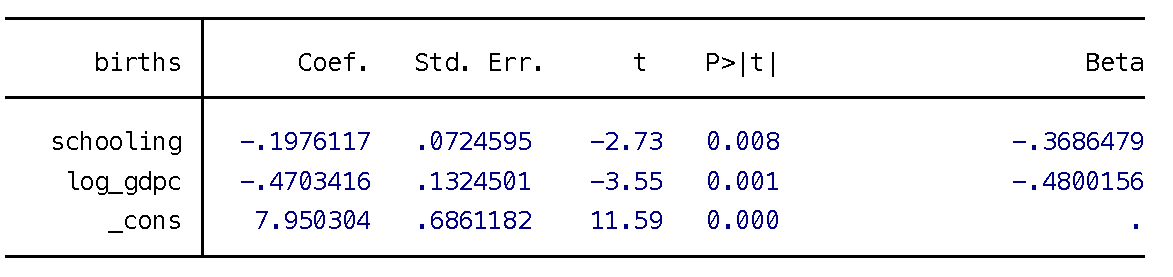
\includegraphics[scale=.45]{mreg-output-beta.pdf}

		\footnotesize{\textit{(identical output for overall model fit omitted)}}
		
		\begin{alertblock}{Sanity check}

			Interpret unstandardized coefficients; use standardization only for model comparisons.

		\end{alertblock}

	\end{frame}

		\section{Regression dummies}

		\begin{frame}[t]{Regression dummies and categorical predictors}

			\begin{block}{Single coefficient of dummy $X_3$}

				\vspace{-1em}
				\begin{align*}
					Y &= \alpha + \beta_1 X_1 + \beta_2 X_2 + \color{gray} \beta_3 (0) \color{fg} + \epsilon \\
					Y &= \alpha + \beta_1 X_1 + \beta_2 X_2 + \red{\beta_3 (1)} + \epsilon
				\end{align*}

				The omitted category $X_3 = 0$ is called the \red{reference category} and is part of the \red{baseline model} $Y = \alpha$, for which all coefficients are null.
				
			\end{block}
			
			\begin{exampleblock}{Example}

				\vspace{-1em}
				\begin{align*}			
					Income &= \alpha + \beta_1 \cdot \text{age} + \beta_2 \cdot \text{education} + \color{gray} 0 \cdot \text{male} \color{fg} & + \epsilon \\
					Income &= \alpha + \beta_1 \cdot \text{age} + \beta_2 \cdot \text{education} + \red{1 \cdot \text{female}} & + \epsilon
				\end{align*}

			\end{exampleblock}
			
		\end{frame}
					
	\begin{frame}[t]{\texttt{reg births schooling log\_gdpc \red{i.region}}}

		Categorical variables can be used as \red{dummies}, i.e. binary recodes of each category that are tested against a \red{reference category} to provide regression coefficients for the net effect of each category:\\[.5em]

		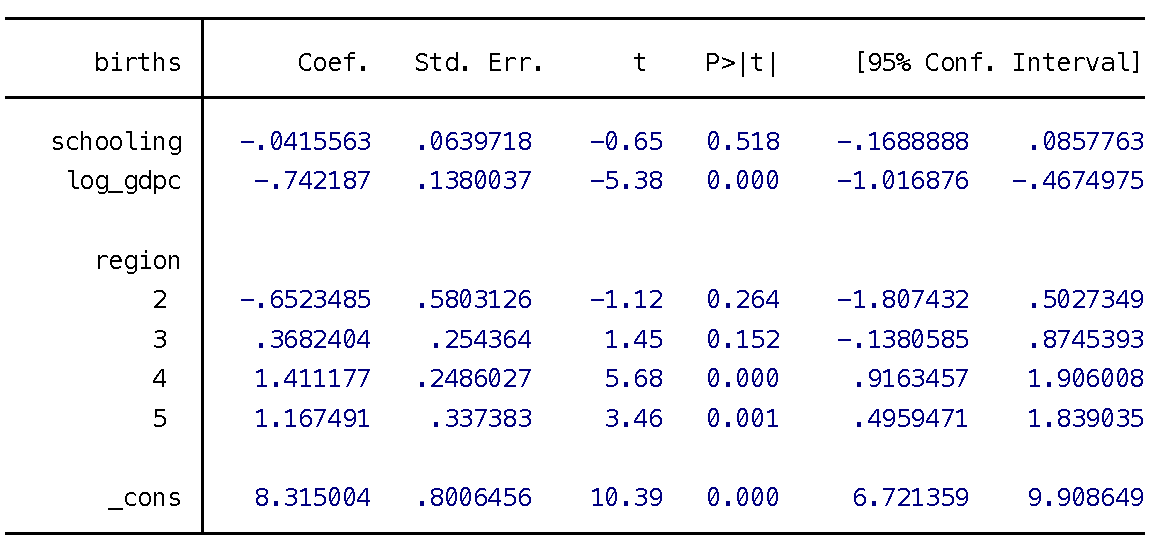
\includegraphics[scale=.45]{mreg-output-dummies.pdf}

		\footnotesize{\textit{(identical output for overall model fit omitted)}}

	\end{frame}

	\section{Regression diagnostics}

	\begin{frame}[t]{Regression diagnostics}

		\begin{block}{Residuals}

			\begin{itemize}
				\item \texttt{predict yhat}: fitted values
				\item \texttt{predict r, resid}: residuals
				\item \texttt{predict r, rsta}: standardized residuals		
			\end{itemize}
			
			Use \texttt{rvfplot} for residuals-versus-fitted values plots.

		\end{block}

		\begin{alertblock}{Heteroskedasticity}

			When the residuals are not normally distributed, the model expresses \red{heterogeneous variance} (unreliable standard errors).

		\end{alertblock}

		\begin{exampleblock}{Examples: \href{http://www.ats.ucla.edu/stat/stata/webbooks/reg/chapter2/statareg2.htm}{UCLA \textit{Regression with Stata}, ch.~2}}

			There are many more diagnostics on display there.

		\end{exampleblock}
		
	\end{frame}

    %
    %
    	
	\begin{frame}[t]{Regression diagnostics}

		\begin{block}{Interaction terms}

			\begin{itemize}
				\item Use \texttt{vif} to detect variables with $VIF > 10$
				\item Use \texttt{\#} and \texttt{\#\#} to capture interactions
				\item Use \texttt{c.} to interact continuous variables
			\end{itemize}
			
			(See also \texttt{avplot} and partial regression.)
		\end{block}

		\begin{alertblock}{Variance inflation}

			Variables that strongly interact induce \red{multicollinearity} `inside' your model, making standard errors unreliable.

		\end{alertblock}

		\begin{exampleblock}{Examples: \href{http://www.ats.ucla.edu/stat/stata/faq/}{UCLA Stata FAQ}}

			Search for ``comparing coefficients across groups''.

		\end{exampleblock}
					
	\end{frame}

    %
    %

%	\section{Final paper}
%
%	\begin{frame}[t]{Final paper}
%	
%	\begin{columns}[T]
%	\column{.3\textwidth}
%	\textbf{Univariate\\statistics}
%	
%	\vspace{.55em}
%	\begin{itemize}
%		\item Introduction
%		% (analysis of survey data)
%		\item Datasets
%		% (observations and variables)
%		\item Distributions
%		% (central tendency, variability, normality)
%		\item Estimation
%		% (PDF, CLT, LLN, CI, MLE)
%	\end{itemize}
%	Assignment No. 1
%	
%	\column{.3\textwidth}
%	\textbf{Bivariate\\statistics}
%	
%	\begin{itemize}
%		\item Significance
%		% (t-test, comparison of means and proportions)
%		\item Crosstabs
%		% (Chi-squared test)
%		\item Correlation
%		% (scatterplot and correlation matrixes)
%		\item Linear regression
%		% (Simple OLS linear regression)
%	\end{itemize}
%	Assignment No. 2
%	
%	$$
%	\left.
%    \begin{array}{rrr}
%        corrected \\
%        revised\\
%        appended
%    \end{array}
%	\right \} 
%	$$
%
%	\column{.3\textwidth}
%	\textbf{Statistical\\modelling}
%	
%	\begin{itemize}
%		\item Basics
%		% (residuals)
%		\item Extensions
%		% (dummies)
%		\item Diagnostics
%		% (multicollinearity, heteroscedasticity)
%		\item Conclusion
%		% (GLS, logistic, ANOVA, Bayesian...)
%	\end{itemize}
%	\red{Final paper}\\[.5em]
%	\fbox{
\includegraphics[width=.75\textwidth]{holy-grail.jpg}}
%	\end{columns}
%	
%	\end{frame}
%	
%	\begin{frame}[t]{Final paper}
%
%		\begin{block}{Essential instructions}
%
%			\begin{itemize}
%				\item Review \red{paper template}: \url{http://goo.gl/7u8oa}
%				\item Respect \red{paragraph limits} mentioned in the template
%				\item Improve \red{formatting} (styles, citations, fonts…)
%			\end{itemize}
%			
%		\end{block}
%
%		\begin{block}{3-step guide}
%
%			\begin{enumerate}
%				\item \red{Rewrite} from top to bottom
%				\item \red{Select} what you report
%				\item \red{Balance} evidence and analysis
%			\end{enumerate}
%
%		\end{block}
%					
%	\end{frame}
%
%	\begin{frame}[t]{Systematic \red{interpretation}}
%		\begin{columns}[T]
%			\column{.5\textwidth}
%			If you forget to interpret your output, you will be thrown into the gaping mouth of the sarlaac that inhabits the Great Pit of Carkoon on planet Tatooine ($p < 0.01$).\vspace{1em}
%			
%			And kittens will get hurt.
%			\column{.4\textwidth}
%			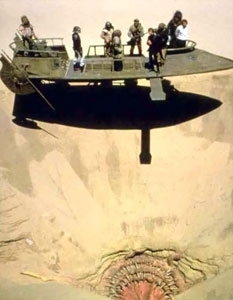
\includegraphics[height=.66\paperheight]{sarlaac.jpg}
%		\end{columns}
%	\end{frame}
%
%	\begin{frame}[t]{Systematic \red{references}}
%		\begin{columns}[T]
%			\column{.5\textwidth}
%			If you forget to reference your sources, the hideous terror of Cthulhu will arise from the sunken city of R'lyeh to spread the abject curse of the Great Old Ones onto this world ($p < 0.01$).\vspace{1em}
%		
%			And kittens will get hurt. Again. Different ones.
%			\column{.4\textwidth}
%			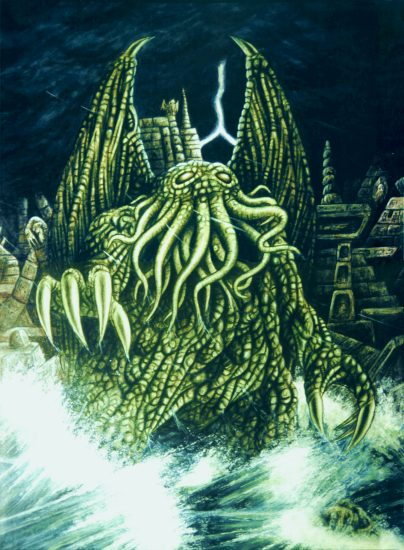
\includegraphics[height=.66\paperheight]{cthulhu.jpg}
%		\end{columns}
%	\end{frame}
%	
%	
%	\begin{frame}[t]{Systematic \red{proofreading}}
%		\begin{columns}[T]
%			\column{.5\textwidth}
%			If you forget to proofread your work, a gigantic hole might open in the earth under your feet, and you might burn in the flames of the monstrous Moloc'h for eternity ($p < 0.01$).\vspace{1em}
%			
%			And your graders will get angry at their laptops.\vspace{1em}
%			
%			All remaining kittens will be decimated without any sign of human mercifulness.
%			\column{.4\textwidth}
%			
\includegraphics[height=.66\paperheight]{explain.jpg}
%		\end{columns}
%	\end{frame}
%	
%    %
%    %
%	
%    \begin{frame}[c]{Thanks for your attention}
%    
%        \begin{alertblock}{Final paper}
%            \begin{itemize}
%                \item Name your paper and do-file like \red{Briatte\_Petev\_final}
%                \item Make sure to print your paper to a slick \red{PDF}
%                \item Email with subject ``\red{SRQM}: Final paper, \textit{[your names]}''
%                \item Do not forget to \red{copy your partner} on all emails
%            \end{itemize}
%        \end{alertblock}
%        
%        \begin{block}{Readings}
%            \begin{itemize}
%                \item \emph{Stata Guide}, Sec.~11 and 13--16
%            \end{itemize}
%        \end{block}
%            
%    \end{frame}
%
%	\begin{frame}[c,plain]
%		\begin{center}
%			
\includegraphics[width=\textwidth]{this-is-stata.jpg}
%		\end{center}
%	\end{frame}
%	
%	\begin{frame}[c,plain]
%			\vspace{.3\paperwidth}
%		\begin{center}
%			{\Large \red{Congratulations}, and thank you.}\\
%		\end{center}
%			\vspace{1em}
%			\hspace{.6\paperwidth}
%			\texttt{exit, clear}		
%	\end{frame}
	
\end{document}
